Dans ce (pas très) court tutoriel, nous allons vous montrer comment 
fabriquer votre propre station météo. Et comme ça serait un peu trop banal, 
votre station météo sera en plus mobile ! Nous proposons pour cela une
architecture assez simple, avec d'un côté une Raspberry Pi qui fera office de
serveur et de gestionnaire, et d'un autre côté une Arduino motorisée faisant
office de station météo.

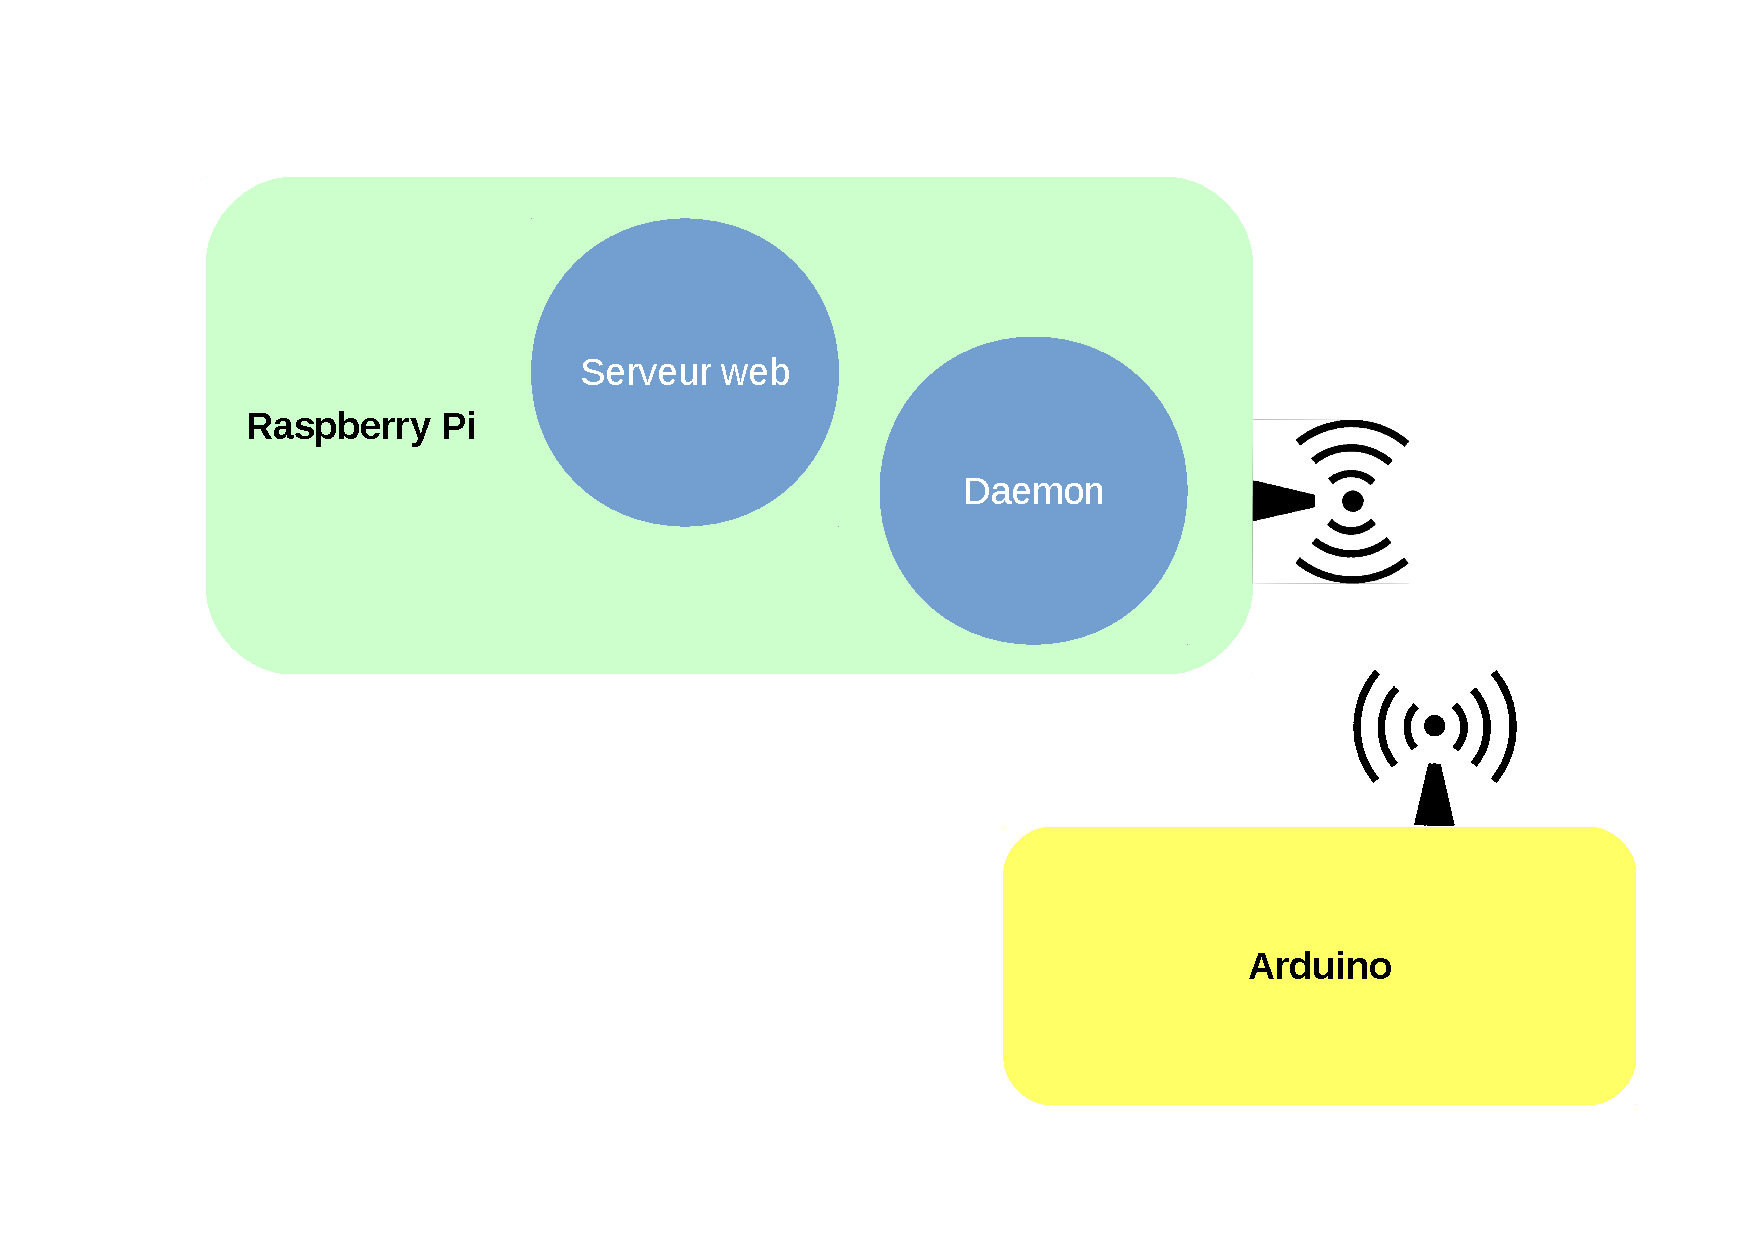
\includegraphics[width=\textwidth]{include/archi.pdf}

On notera que la Raspberry contient deux entités : le serveur web, qui permettra
de tout gérer de l'extérieur, et le daemon, qui fera le lien entre le serveur 
web et l'Arduino par le biais de communications radios.
